\chapterimage{back2.jpg} % Chapter heading image
\chapter{Architecture and Safety Principles}

\section{Introduction to safety}
Safety critical systems are systems where life is at risk. One \textit{mistake} could lead to injury or death (of passengers aboard trains, planes, or cars for example).\\

\noindent One question for a developer is: 
\begin{center}
"would you dare to execute your program if someone would die in case of a crash / core dump / fatal error / etc. especially someone you know like a friend or a member of your family?"    
\end{center}

\begin{figure}[h]
\centering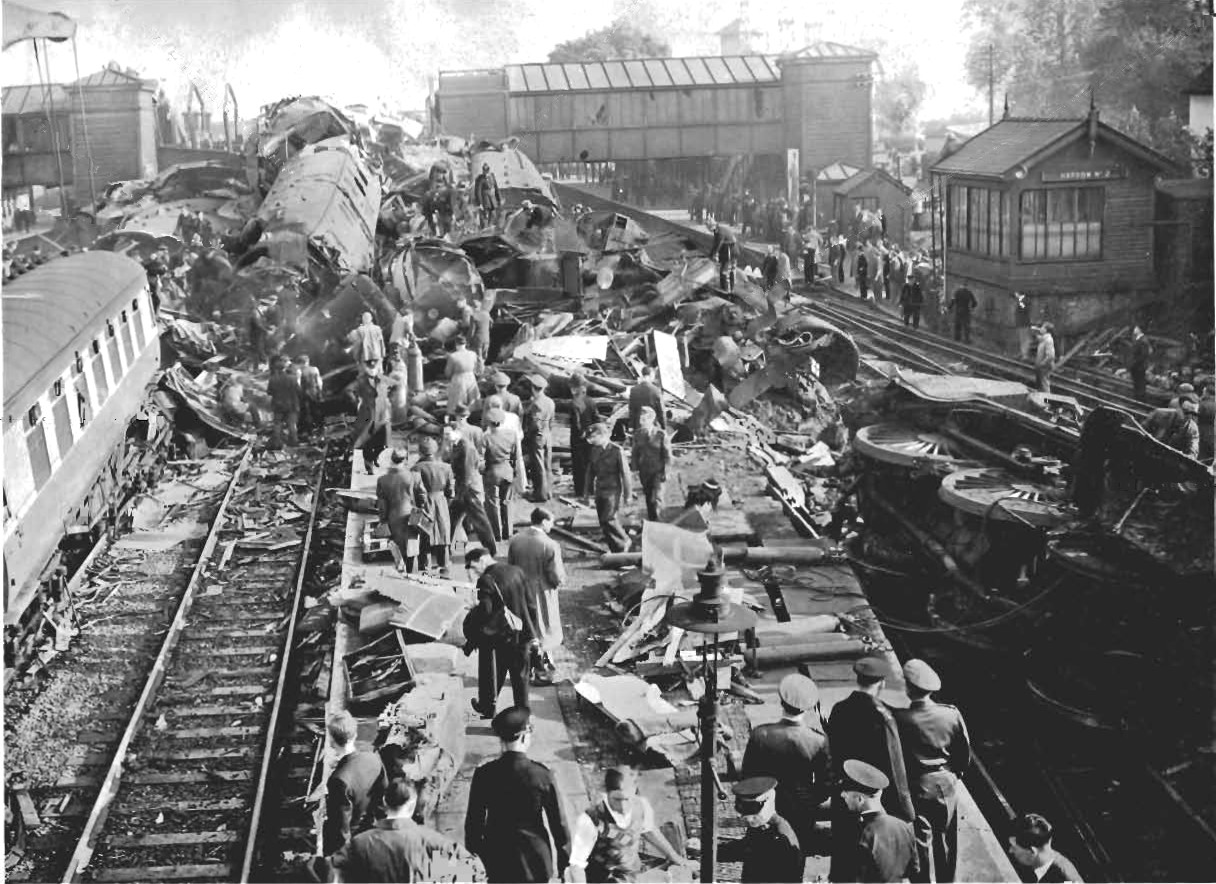
\includegraphics[scale=0.2]{Pictures/chapterSafetyPrinciples/SAFETY-crash.jpg}
\caption{Double collision which occurred on 8th October 1952 at Harrow and Wealdstone Station}
\end{figure}

When you develop a safety system, you are not left alone. Depending on your application domain, you have standards that provide you guidance based on the safety level you are looking for. Note that these standards do not provide a definitive recipe to produce safety systems, but more a collection of state-of-the-art recommendations related to the software, hardware, and development process \footnote{and also maintenance}.

\begin{figure}[h]
\centering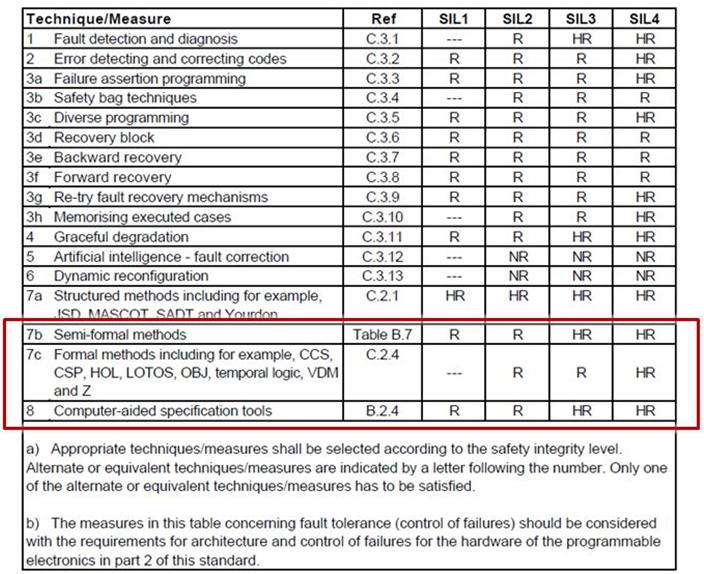
\includegraphics[scale=0.5]{Pictures/chapterSafetyPrinciples/SAFETY-61508A-2.png}
\caption{Table from IEC 61508 standard showing design recommendations for SIL1 to SIL4 software (R: recommended, HR: highly recommended, NR: not recommended. Note that nothing here, including formal methods, is mandatory}
\end{figure}

Before connecting your system to the real world and switching it on, you need to complete a safety case, that is a demonstration the feared event(s)\footnote{in the railway sector, it is mainly train collision} will not happen more frequently than expected. For SIL3, it is one failure every 100 years, and for SIL4, one failure every 10,000 years. \\ 

For the safety case, you need to consider the whole picture: the hardware (computers, sensors, actuators, etc.), the software, and the environment at large. The main question is: 
\begin{center}
    "what could happen in case that something fails?"
\end{center}
We are far from the concept: "it compiles, hence it works". The safety case always depends on a number of hypotheses that restrict the scope. The idea is not to protect against everything but only to consider a set of "reasonable" situations. As an example, for train collision, we do not consider a plane that could crash on the tracks.\\

\noindent The "failures" considered are diverse and represent a large spectrum of situations: 
\begin{itemize}
    \item specification error: we specified the wrong system or software.
    \item development error: the specification is correct but the implementation does not comply with its specification. It could be a functional mistake: the algorithm is doing something different than what is expected. It could be non-functional: the operation is performed slower than expected.
    \item programming error: numbers are divided by 0, arithmetic computation produces overflow, or tables are accessed outside of their range.
    \item compilation error: binary code produced does not comply with source code \footnote{Who is reading the binary code these days?}
    \item wrong execution: the memory is corrupted (wrong data, wrong instruction, corrupted program counter), the hardware is failing (wrong instruction execution, incorrect storage/access)
    \item failing hardware: sensors are providing incorrect values, actuators cannot be commanded properly.
\end{itemize}

For a SIL4 system, the target reliability is between $10^{-7}$/h to $10^{-9}$/h. Given that a processor reliability is estimated between $10^{-4}$/h to $10^{-6}$/h, a single processor is not sufficient for a SIL3 or SIL4 system. That is why two processors (or more) are used in parallel (traditionally with a voter - the two processors have to come to the same decision to initiate a potentially risky action \footnote{for example, opening platform screen doors on a metro platform with the risk that waiting passengers could fall on the tracks if no train is present.}). In addition, the two processors are equipped with protecting mechanisms that would allow the system to continue its mission in case of perturbation / failure.  



\begin{figure}[h]
\centering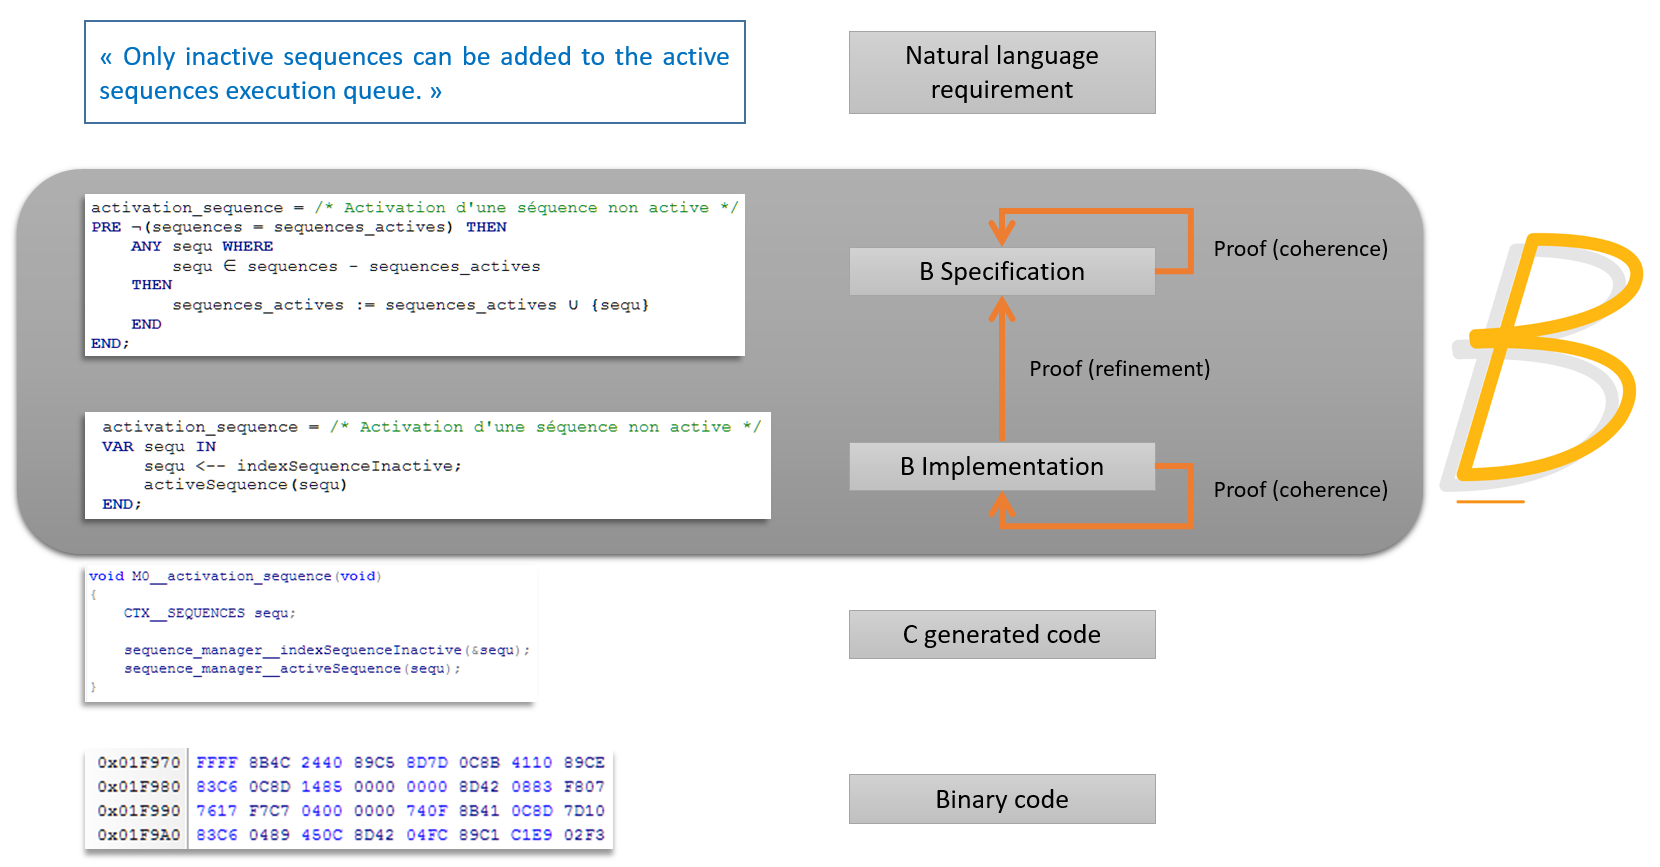
\includegraphics[scale=0.3]{Pictures/chapterSafetyPrinciples/SAFETY-Bcycle.png}
\caption{Path from requirements to binary code with B}
\label{safety:B}
\end{figure}

The contribution of B to the safety case is explained in figure \ref{safety:B}. In this figure, we see the different stages from requirements to binary code (from top to bottom). The B method covers the software specification and implementation stages (the grey box) where the specification and implementation models are proved (we will see later on what it means). However the inputs and outputs of this grey box are error prone:
\begin{itemize}
    \item the specification model could be different from the natural language requirements. Usually human based cross verification is required - every requirement should be in the model, every modelling element should be issued from the natural language requirements. Validation testing also helps to find mistakes at this stage.
    \item the code generated could be different from the implementation model: the code generator may alter the semantics of the implementation model due to incorrect code generator specification or bugs.
    \item the binary code could be different form the source code: the compiler may alter the semantics of the source code, due to improper optimisation options or bugs.
    \item the processor executing the binary code could exhibit a misbehaviour due to either internal reasons (design or production flaw) and/or external reasons (high energy particles, electromagnetic waves, etc.).\\
\end{itemize}

Usually the last three bullets are taken into account with diversity, given that the program is executed on two (or more) processors: two different code generators are used to produce two different source codes from the same formal model. It is very unlikely that two tools developed with different technologies (programming language, libraries, compiler) and by independent teams are going to exhibit the same unsafe behaviour under the same conditions. One code generator could for example use a big endian memory model while the other uses a little endian one. Another option is to add void instructions \footnote{One code could be xx := yy + zz while the other is xx := yy + zz + 1 - 1 } in one source code only that do not change the final behaviour but produce a different binary code. That way a processor perturbation would not affect the two programs the same way because different parts of each program are being executed.\\

We can clearly see that in the case of safety systems, the B method is only one part of the story and other means have to be set up in order to reach safety related objectives. These means require rare human resources to complete successfully because of the deep level of understanding of both hardware and software parts to consider. \\

\begin{figure}[h]
\centering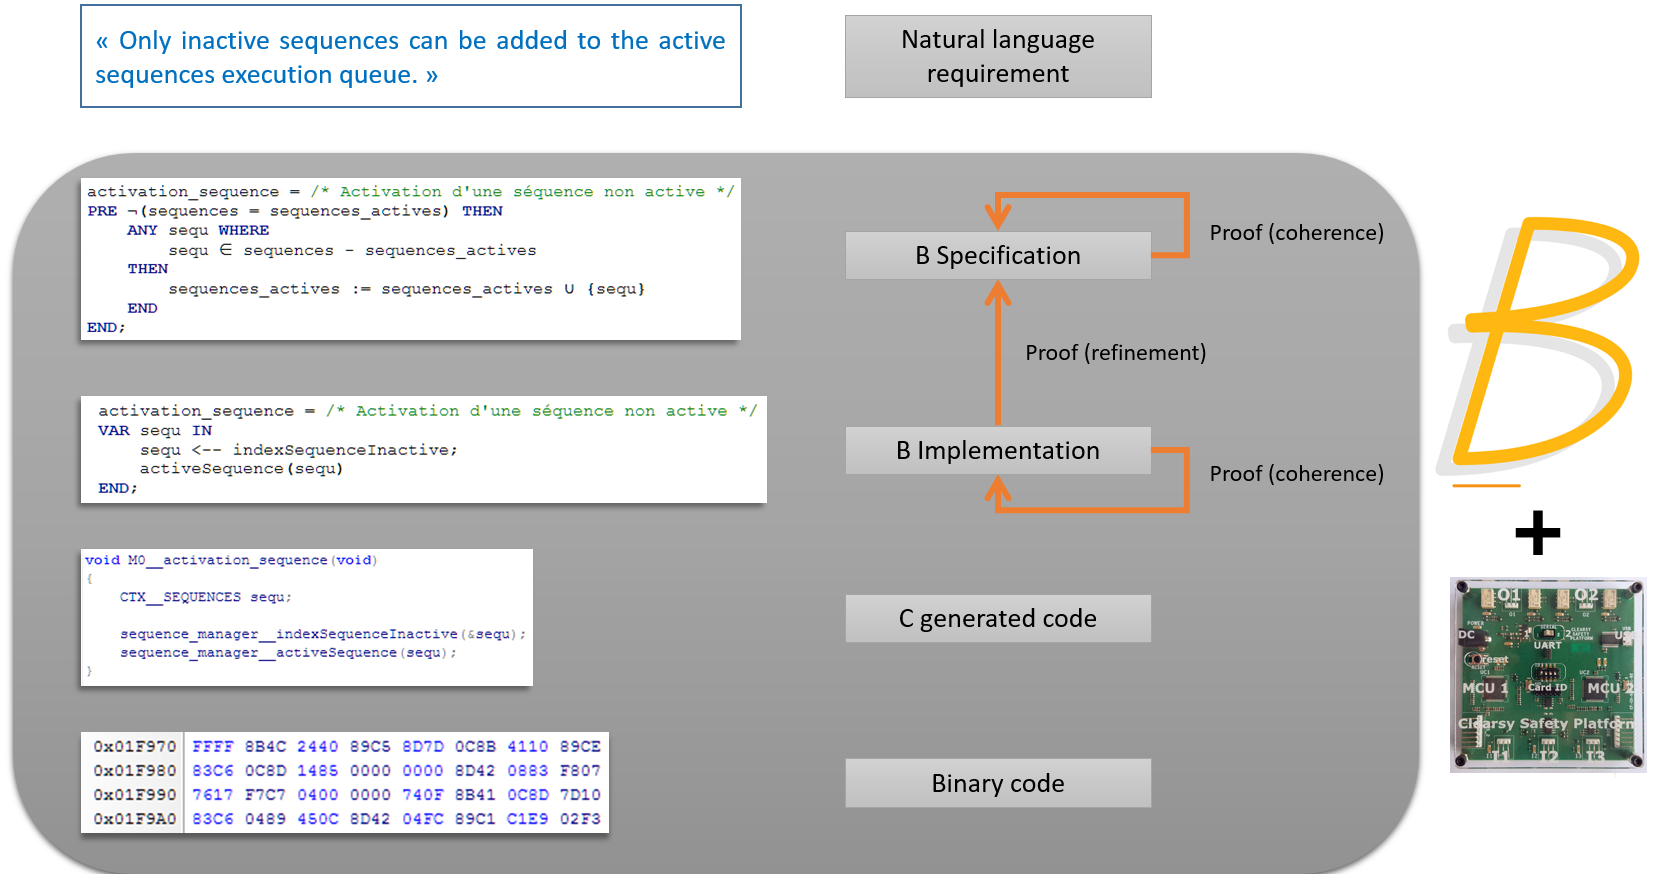
\includegraphics[scale=0.3]{Pictures/chapterSafetyPrinciples/SAFETY-BCSSPcycle.png}
\caption{Path from requirements to binary code with B with the CLEARSY Safety Platform}
\label{safety:CSSP}
\end{figure}

With the CLEARSY Safety Platform, the very technical aspects related to safety are taken into account by the platform (see chapter \ref{safety:safety-principles}), leaving the developer to focus only on the development of the function to perform. In the figure \ref{safety:CSSP}, the combination of B and CSSP covers all the steps from software specification to binary code. The developer is only required to be able to specify and program in B (with DSL if a translator from DSL to B is available), thus less expert profiles could be used for the development. The only remaining activity to perform (apart from validation testing, always mandatory) is the traceability/coverage between natural language requirement and formal modelling. Hence the CLEARSY Safety Platform, with its technology based on a double processor and a formal method with proof to ensure safety at the highest level, fulfils the need for a technical solution to overcome the difficulties of developing SIL3/SIL4 systems.

\section{Architecture}

The CLEARSY Safety Platform  is made of two parts: an IDE to develop the software and an electronic board to execute this software. The full process is described in figure \ref{arch:principes}.

\begin{figure}[h]
\centering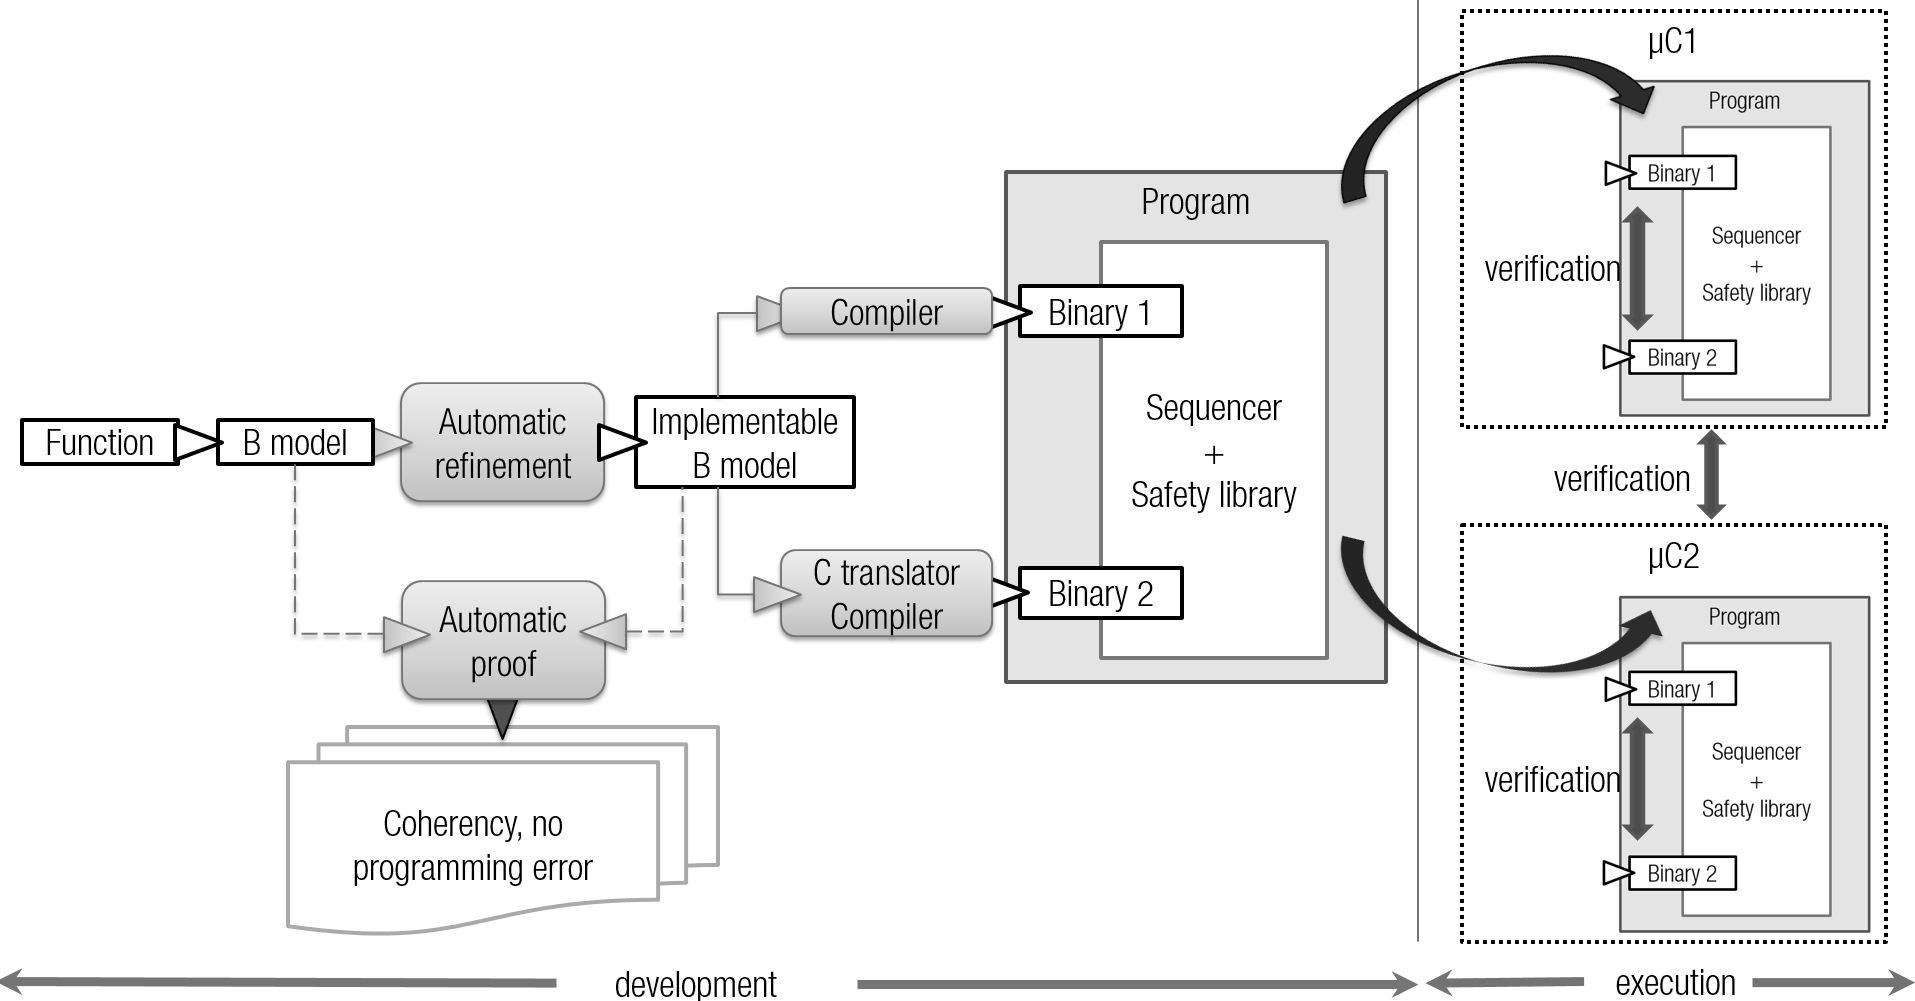
\includegraphics[scale=0.24]{Pictures/chapterSafetyPrinciples/ARCH-LCHIP-principe.jpg}
\caption{Full path from function description to safe execution with the CLEARSY Safety Platform. Round boxes are tools, rectangular boxes are files.}
\label{arch:principes}
\end{figure}

It starts with the function specification (natural language) to develop. The developer has to provide a B model of it (specification and implementation) using the schema:
\begin{itemize}
    \item the function to program is a loop, where the following steps are performed repeatedly in sequence:
\begin{itemize}
    \item the inputs are read \footnote{Inputs are similar for $\mu C_1$ and $\mu C_2$, unless the inputs are captured at different times in which case the different values would cause the platform to enter panic mode.}
    \item some computation is performed
    \item the outputs are set
\end{itemize}
\item The steps related to inputs and outputs are fixed and cannot be modified. 
\item Only the computation may be modified to obtain the desired behaviour.\\
\end{itemize}


The implementation is usually handwritten but could also be generated automatically with the B Automatic Refinement Tool \footnote{However automatic refinement requires a higher level of experience of B and is not covered in this book.}. The B models are proved (mostly automatically as the level of abstraction of typical command \& control applications is low) to be coherent and to contain no programming error.
From the implementable model, two binaries are generated:
\begin{itemize}
    \item binary$_1$, obtained via a dedicated compiler (developed by CLEARSY) transforming a B model into HEX \footnote{"Intel HEX is a file format that conveys binary information in ASCII text form. It is commonly used for programming microcontrollers, EPROMs, and other types of programmable logic devices." (Wikipedia)} file,
    \item binary$_2$, produced with the Atelier B C code generator then compiled with the GCC compiler into another HEX file.
\end{itemize} 
Each binary represents the same function but is supposed to be made of different sequences of instructions because of the diversity of the tool chains. 
Then the two binaries binary$_1$ and binary$_2$ are linked with:
\begin{itemize}
    \item a sequencer, in charge of reading inputs, executing binary$_1$ then binary$_2$, and setting the outputs
    \item a safety library, in charge of performing safety verification (more details in chapter \ref{safety:safety-principles}). In case of failing verification, the board enters panic mode, meaning the outputs are deactivated \footnote{No power is provided to the Normally Open (NO) outputs, so the output electric circuits are open.}, the board status LED start flashing, and the board enters an infinite loop doing nothing. A hard reset (power off or reset button) is the only possibility to interrupt this panic mode.
\end{itemize}
The final program is thus made of binary$_1$, binary$_2$, the sequencer and the safety library. The memory mappings of binary$_1$ and binary$_2$ are separate. 

This program is then uploaded on the two micro-controllers $\mu C_1$ and $\mu C_2$. The bootloader, on the electronic board, checks the integrity of the program (CRC, separate memory spaces). Then both micro-controllers start to execute the program. During its execution, the following are performed:
\begin{itemize}
    \item internal verification:
\begin{itemize}
    \item every cycle, binary$_1$ and binary$_2$ memory spaces (variables) are compared
    \item regularly, binary$_1$ and binary$_2$ memory spaces (program) are compared \footnote{This verification is performed "in the background" over thousands/millions of cycles, to keep a reasonable cycle time.}
    \item regularly, the identity between memory output states and physical output states is checked to detect if the board is unable to command the outputs.
\end{itemize} 
\item external verification:
\begin{itemize}
    \item regularly (every 50ms at the latest), memory spaces (variables) are compared between $\mu C_1$ and $\mu C_2$. 
\end{itemize} 
\end{itemize} 
If any of these verifications fail, the board enters the panic mode.

The whole process is fully supported by adequate tools. In the figure \ref{arch:process}, the tools and text/binary files generated are made explicit for both the application (path used every time an application is developed) and the safety belt (developed once for all by the IDE development team \footnote{Note that from the abstract formal model, one part of the software is developed in B with concrete formal model, while the other part is developed manually. It happens when using B provides no added-value (for example low-level IO). A component modelled in B and implemented manually is called a basic machine.}. The tools are issued from Atelier B, except:
\begin{itemize}
    \item the B to HEX compiler, initially developed to control platform screen doors for metro lines in Brazil. This tool proceeds in two steps: a translation from B to ASM MIPS, then from ASM MIPS to HEX \footnote{In order to ease debugging as ASM MIPS to HEX is a straightforward line-to-line translation.}.
    \item the C to HEX GCC compiler.
    \item the linker combining the 2 hex files with the safety sequencer and libraries.
    \item the bootloade.r\\
\end{itemize}



We can clearly see that the CLEARSY Safety Platform is a generic PLC \footnote{"A Programmable Logic Controller is an industrial digital computer which has been ruggedized and adapted for the control of manufacturing processes, such as assembly lines, or robotic devices, or any activity that requires high reliability control and ease of programming and process fault diagnosis." (wikipedia)} able to perform command and control over inputs and outputs. The overall architecture is similar between all instances of the CLEARSY Safety Platform. The differences are due to the physical interface:
\begin{itemize}
    \item 5 IOs for SK$_0$, 28 for SK$_1$.
    \item digital (Boolean) IOs for SK$_0$ and SK$_1$, analog IOs in the future.
    \item network connection (messaging) through a maintenance processor, in the future.
\end{itemize}

\begin{remark}
From a safety point of view, the current architecture is valid for any kind of mono-core processor. The decision of using PIC32 micro-controllers (able to deliver around 50 DMIPS) was made based on our knowledge and experience of this processor. Implementing the CLEARSY Safety Platform on other hardware \footnote{STM32 for example} would "only" require the existing electronic board and software tools to be modified, without impacting much the safety demonstration.
\end{remark} 

\begin{figure}[h]
\centering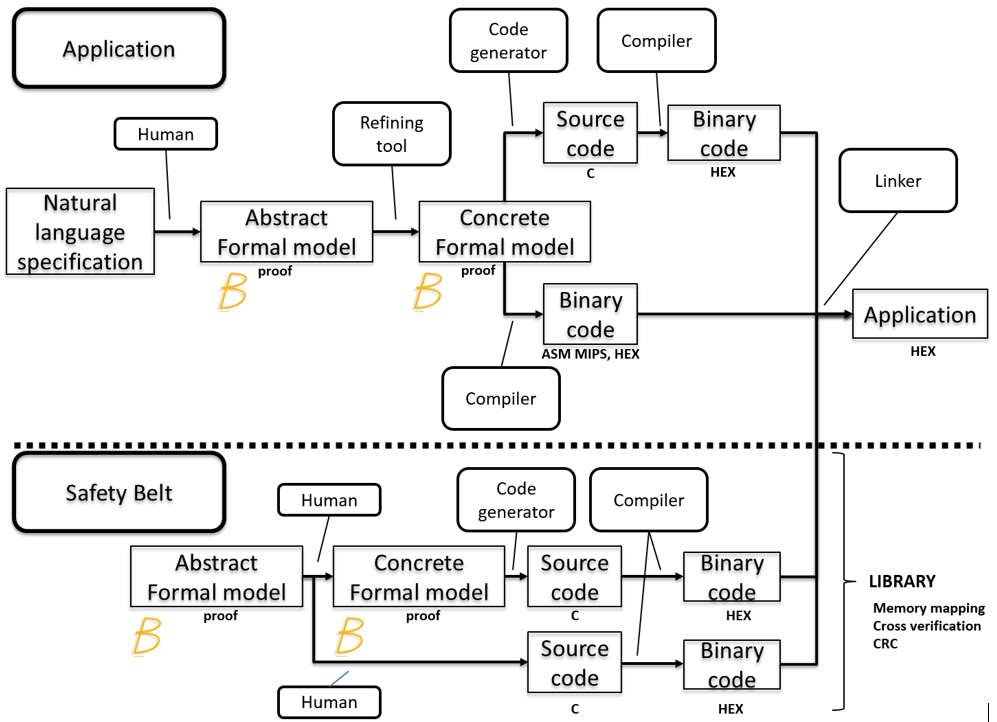
\includegraphics[scale=0.35]{Pictures/chapterSafetyPrinciples/ARCH-LCHIP-process.jpg}
\caption{Tools and files involved in the generation of the software}
\label{arch:process}
\end{figure}



\section{Safety Principles}
\label{safety:safety-principles}

The safety is built on top of few principles:
\begin{itemize}
    \item a B formal model of the function to develop, proved to be coherent, to correctly implement its specification, and to be programming error-free,
    \item four instances of the same function running on two micro-controllers (two per micro-controller with different binaries obtained from diverse tool-chains) and the detection of any divergent behaviour among the four instances,
    \item the deferred cross-verification of the programs on the two $\mu C$,
    \item outputs require both $\mu C_1$ and $\mu C_2$ to be alive and running as one provides energy and the other one the command,
    \item output physical states are regularly verified to comply with the memory states, to check the ability of the board to command its outputs,
    \item input signals are continuous (0 or 5V) and are made dynamic (addition of a frequency signal) in order to prevent the short-circuit current from being considered  as high level (permissive) logic.
\end{itemize}

\begin{table}[ht]
\small
\begin{tabular}{|l|c|l|l|}
\hline
\textbf{Stage} & \textbf{\#} &  \textbf{Failure}                  & \textbf{CSSP verification} \\ \hline
specification  & 1 & Typing error                      & Typechecker tool detects typing error \\ \hline
specification  & 2 & Specified behaviour incompatible  & Unprovable proof obligation indicates   \\
               & & with invariant properties         & specification mistake       \\ \hline           
implementation & 3 & Typing error                      & Typechecker tool detects typing error \\ \hline
implementation &   & Implemented behaviour incompatible  & Unprovable proof obligation indicates   \\
               &   & with invariant properties         & implementation mistake       \\ \hline           
implementation & 4 & Implemented behaviour incompatible  & Unprovable proof obligation indicate   \\
               &   & with specified behaviour          & implementation mistake       \\ \hline 
implementation & 5 & Overflow capable arithmetic operators  & Detected by the B-to-HEX compiler   \\
               &   & used instead of dedicated ones     &       \\ \hline 
implementation & 6 & IF clause with more than one condition  & Detected by the B-to-HEX compiler   \\
               &   & (B0 language restriction)          &       \\ \hline 
implementation & 7 & LOCAL variables not typed before use  & Detected by the B-to-HEX compiler   \\
               &   & (B0 language restriction)          &       \\ \hline                
code generation & 8 & Syntax errors in the C generated code  & Detected by the MICROCHIP compiler   \\  \hline
code generation & 9 & Incorrect naming in the C         & Detected by the linker   \\            
                &   & generated code                    &           \\ \hline  
code generation & 10 & Incorrect memory map             & Memory overlap detected by the   \\  
                &    &                                 &  bootloader   \\ \hline 
\end{tabular}
\caption{Verification performed during development}
\label{safety:verif-dev}
\end{table}     
 However, as explained in the chapter \ref{preface}, the electronic board lacks some vital elements to comply with highest SIL requirements like:
 \begin{itemize}
     \item ensure galvanic isolation between the two half-boards, to prevent that one side of the board wrongly provides energy to the other side's outputs,
     \item activate safety outputs with a sinusoidal signal \footnote{The micro-controller needs to be alive to generate the sinusoidal signal.} instead of a continuous signal, to ignore fault current and activate output.
 \end{itemize}
These missing features are only needed for real-life safety critical systems and do not prevent developers, whether students, researchers or engineers, from using the CLEARSY Safety Platform for education and prototype development. 

The verification performed by the CLEARSY Safety Platform, either during development or execution stages, is summarised in tables \ref{safety:verif-dev} and \ref{safety:verif-exec}.
\begin{table}[ht]
\small
\begin{tabular}{|l|c|l|l|}
\hline
\textbf{Stage} & \textbf{\#} &  \textbf{Failure}                  & \textbf{CSSP verification} \\ \hline                
compilation    & 11 & Wrong binary code generated       & Detected during execution by safety \\
               &    &                                   & library by comparing binary$_1$ and  \\ 
               &    &                                   &  binary$_2$ variables in memory\\ 
               &    &                                   & with CRC on the same $\mu C$ \\ \hline
uploading      & 12 & Incorrect transfer between host   & Detected by bootloader during upload (CRC)\\
               &    & and electronic board              & and during execution over several cycles\\ \hline

execution      & 13 & RAM error (variables)             & Detected by comparing binary$_1$ \\
               &    &                                   & and binary$_2$ variables in memory \\
               &    &                                   & with CRC on the same $\mu C$ \\ \hline
execution      & 14 & RAM error (program)             & Detected by comparing binary$_1$ \\
               &    &                                   & and binary$_2$ program in memory \\
               &    &                                   & with CRC with the other $\mu C$ \\ \hline
execution      & 15 & Failure of one $\mu C$        & Detected by handshake between $\mu C_1$  \\ 
               &    &                               & and $\mu C_2$ at least every 50 ms \\ \hline
execution      & 16 & Outputs not command-able       & Detected by checking physical state  \\ 
               &    &                               & and command issued by the software \\
\hline
\end{tabular}
\caption{Verification performed during execution}
\label{safety:verif-exec}
\end{table}




